\documentclass{beamer}
\setbeamertemplate{section in toc}[sections numbered]
\usefonttheme[onlymath]{serif}
\usepackage{amsmath}
\usepackage{graphicx}
\usepackage{subfigure}
\usepackage{lmodern}
\usepackage{amsmath}
\usepackage{braket}
\usepackage{color}
\usepackage{bm}
\usepackage{amssymb}
\usepackage{tikz}
\usepackage{tikz-cd}
\usetikzlibrary{matrix,calc,arrows,patterns,angles,quotes,shapes.geometric,positioning}
\newcommand{\blue}[1]{{\color{blue}{#1}}}

%Information to be included in the title page:
\title{Antiferromagnetic Spin Chains}
%\author{Ammar Jahin}
%\institute{University of Florida}
\date{University of Florida, April 2020}

\begin{document}
\frame{\titlepage 

    This talk follows the review by I Affleck 1989 J. Phys.: Condens. Matter 1 3047
    
    }

\section*{Introduction}
\begin{frame}
    \frametitle{Introduction}
    The problem at hand is to study whether a 1D antiferromagnetic system ia gapped or not. \pause 

    Review of what we know about spin systems and long range order that can help us answer this problem: \pause
    \begin{enumerate}
        \item Mermin-Wagner theorem, no long range order in 1D. \pause 
        \begin{itemize}
            \item Doesn't imply the existence of a gap. Something like a BKT phase might occur. \pause
            \item  Can only tell us about long range order at finite temperature. Not much about the ground state. In a sense our question is more elementary, it's about the nature of the ground state itself. \pause 
        \end{itemize} 
        \item Goldstone modes, and spin-wave theory. \pause 
        \begin{itemize}
            \item Using the Neel state as the broken symmetry state one might think we should be able to find spin-wave excitations which we know are gapless, and lead to power law correlations.  
        \end{itemize}
    \end{enumerate}
    

\end{frame}

\begin{frame}
    \frametitle{Outline}
    \tableofcontents
\end{frame}

\AtBeginSection[]
{
\begin{frame}
    \frametitle{Outline}
    \tableofcontents[currentsection]
\end{frame}
}



\section{Spin-waves for 1D AFM}

\begin{frame}
    \frametitle{Heisenberg model}
    For a 1D chain with local spin-s on each site the Heisenberg Hamiltonian can be written as:
    \begin{align*}
        H &= J \sum_i \vec{S}_{i} \cdot \vec{S}_{i+1} \nonumber \\
          &= J \sum_i S^+_i S^-_{i+1} + S^-_i S^+_{i+1} + S^z_i S^z_{i+1}, 
    \end{align*}
    with 
    \begin{align*}
        S^+ = \frac{1}{\sqrt{2}} \left(S^x + i S^y \right) && S^- = \frac{1}{\sqrt{2}} \left(S^x - i S^y \right), \nonumber \\
        [ S^i, S^j  ] = i \epsilon^{ijk} S^k && [ S^+, S^-] = S^z
    \end{align*} 
    \pause
    \begin{columns}
    \begin{column}{0.5\textwidth}
        Ferromagnetism: 
        $J<0$ 
        \begin{align*}
            &\ket{\Psi_{\text{FM}}} = \ket{ +s\ +s\ +s\dots} \nonumber \\ 
            &H \ket{\Psi_{\text{FM}}} = E_0 \ket{\Psi_{\text{FM}}} \nonumber \\ 
            &\ket{\Psi_0} = \ket{\Psi_{\text{FM}}} 
        \end{align*}
    \end{column}\pause
    \begin{column}{0.5\textwidth}
        Anti-ferromagnetism: 
        $J<0$ 
        \begin{align*}
            &\ket{\Psi_{\text{Neel}}} = \ket{ +s\ -s\ +s\dots} \nonumber \\ 
            &H \ket{\Psi_{\text{Neel}}} \neq E_0 \ket{\Psi_{\text{Neel}}} \nonumber \\ 
            &\ket{\Psi_0} \neq \ket{\Psi_{\text{Neel}}} 
        \end{align*}
    \end{column}
    \end{columns}

\end{frame}


\begin{frame}
    \frametitle{Classical limit in the AFM case}
    The question then becomes: How close is the Neel state to the ground state?\pause

    We notice that, 
    \begin{align*}
        \braket{\Psi_{\text{Neel}}| S^+_i S^-_{i+1} | \Psi_{\text{Neel}}} \propto s \\
        \braket{\Psi_{\text{Neel}}| S^z_i S^z_{i+1} | \Psi_{\text{Neel}}} \propto s^2.
    \end{align*}
    Hence in the classical limit, $s \rightarrow \infty$, one might expect the Neel state to approaches the ground state. \pause 

    Neel state spontaneously breaks the symmetry and hence would result in a Goldstone modes leading to a gapless excitations. 

\end{frame}

\begin{frame}
    \frametitle{Holstien-Primakov transformation in AFM case}
    \begin{columns}
    \begin{column}{0.6\textwidth} 
        \begin{align*}
            S^z_A = s - a^\dagger a && S^-_A = a^\dagger \left[ s-\frac{a^\dagger a}{2} \right]^{1/2}   \nonumber \\ 
            S^z_B = -s + b^\dagger b && S^+_B = b^\dagger \left[s-\frac{b^\dagger b}{2}  \right]^{1/2}
        \end{align*}
    \end{column}
    \begin{column}{0.4\textwidth}
        \begin{figure}[h]
            \centering
            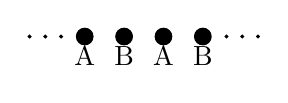
\begin{tikzpicture}[>=triangle 60]
                \foreach \i in {0,...,1}
                {
                \draw[fill, black] (\i,0) circle (3pt) node[anchor=north] {A};
                \draw[fill, black] (\i+0.5,0) circle (3pt) node[anchor=north] {B};
                }
                \foreach \i in {0,...,2}
                {
                \draw[fill, black] (-0.3 - 0.2*\i,0) circle (0.5pt);
                \draw[fill, black] (1.8 + 0.2*\i,0) circle (0.5pt);
                }
            \end{tikzpicture}
            \caption{AB lattice, artificially doubling the unit cell. We put the distance between 2 A sub-lattices to be 1. Let length of the entire chain be $L$.}
            \label{AB_lattice}
        \end{figure}
    \end{column}
    \end{columns}
    with
    \begin{align*}
        [a,a^\dagger] = 1 && [b,b^\dagger] = 1 && [a,b] = 0 && [a,b^\dagger] =0
    \end{align*}
\end{frame}

\begin{frame}
    \frametitle{Classical limit in the AFM case}
    Expanding around a Neel state, using $1/s$ as a small parameter. 
    \begin{align*}
        S^z_A = s - a^\dagger a && S^-_A = \sqrt{s}\  a^\dagger   \nonumber \\ 
        S^z_B = -s + b^\dagger b && S^+_B = \sqrt{s}\  b^\dagger
    \end{align*}
    Using this and after Fourier transforming, dropping a constant term, and keeping only terms of order $O(s)$,
    \begin{align*}
        a_i = \sqrt{\frac{1}{L}} \sum_k e^{ik R_i} a_k && b_i = \sqrt{\frac{1}{L}} \sum_k e^{ik (R_i+1/2)} b_k 
    \end{align*}
    \begin{align*}
        H = 2Js \sum_k  a^\dagger_k a_k + b^\dagger_k b_k + \cos(k/2) a_k b_{-k} + \cos(k/2) b^\dagger_{-k} a^\dagger_k 
    \end{align*}


\end{frame}

\begin{frame}
    \frametitle{Bogoliubov transformation}
    The Bogoliubov transformation, 
    \begin{align*}
        c_k = u_k a_k -v_k b^\dagger_{-k} \nonumber \\
        d_k = u_k b_k - v_k a^\dagger_{-k} \nonumber \\ 
        |u_k|^2 - |v_k|^2 = 1
    \end{align*}
    diagonalize the Hamiltonian, 
    \begin{align*}
        H = 2Js\left[ 1-\cos(k/2) \right]^{1/2} (c^\dagger_k c_k + d^\dagger_k d_k)
    \end{align*} 
    \begin{columns}
    \begin{column}{0.6\textwidth}
        \begin{figure}[h]
            \centering
            \includegraphics[scale=0.25]{tmp_8wmjqz4x.png}
            %\caption{Energy spectrum of AFM spin-waves.}
            \label{spinwave_energy}
        \end{figure}
    \end{column}
    \begin{column}{0.4\textwidth}
        \textbf{Have we shown that the chain is gapless?}
    \end{column}
    \end{columns}
\end{frame}

\begin{frame}
    \frametitle{What goes wrong?}
    \pause
    This approximation only works if the ground state is close to the Neel state.
    The ground state defined as,
    \begin{align*}
        c_k \ket{\Psi_0} = 0 \nonumber \\ 
        d_k \ket{\Psi_0} = 0
    \end{align*}
    \pause 

    This can be checked by comparing $\braket{S^z}$ in the ground state to that of the Neel state, 
    \begin{columns}[T]
    \begin{column}{0.35\textwidth}
        \begin{align*}
            \braket{\Psi_{\text{Neel}}|S^z_i|\Psi_{\text{Neel}}} = \pm s
        \end{align*}
        Remember, 
        \begin{align*}
        S^-_A = a^\dagger \left[ s-\frac{a^\dagger a}{2} \right]^{1/2} 
        \end{align*}
    \end{column}
    \begin{column}{0.65\textwidth}
        \begin{align*}
            \braket{\Psi_0|S^z_i|\Psi_0} = \pm s + \int dk \frac{1}{2} \left[  \frac{1}{|\sin(k)|} - 1\right] 
        \end{align*}
        \alert{\textbf{The correction in infinite for any s.}}
    \end{column}
    \end{columns}
    
\end{frame}

\section{Lieb-Shultz-Mattis theorem}

\begin{frame}
    \frametitle{LSM theory}
    \begin{block}{Statement of the theorem:}
        Any half integer spin chain that is symmetric under parity is either gapless or has a degenerate ground state that breaks parity. 
    \end{block}
    \pause 

    Construct a state $\ket{\Psi_1} = \hat{\eta} \ket{\Psi_0}$ with, 
    \begin{align*}
        &\hat{\eta}  = R^z(\{ \theta_i\}) = e^{i\sum_{i = -l}^{l} \theta_i S^z_i} \ \text{(rotation about odd number of local $z$-axes)} \nonumber \\ 
        &\theta_i = \frac{R_i+l}{l} \pi
    \end{align*}
    \begin{figure}[h]
        \centering
        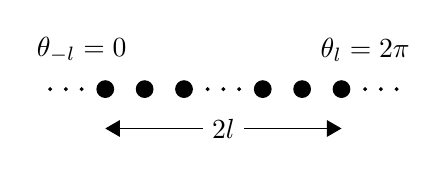
\begin{tikzpicture}[>=triangle 60]
            \foreach \i in {0,...,2}
                {
                \draw[fill, black] (0.5*\i,0) circle (3pt);
                \draw[fill, black] (0.5*\i + 2,0) circle (3pt);
                }
                \foreach \i in {0,...,2}
                {
                \draw[fill, black] (-0.3 - 0.2*\i,0) circle (0.5pt);
                \draw[fill, black] (1.3 + 0.2*\i,0) circle (0.5pt);
                \draw[fill, black] (3.3 + 0.2*\i,0) circle (0.5pt);
                }
                \draw[arrows = <->,black] (0,-0.5)--(3,-0.5);
                \node[rectangle, fill = white] at (1.5,-0.5) {$2l$};
                \node at (-0.3,+0.5) {$\theta_{-l} = 0$};
                \node at (3.3,+0.5) {$\theta_l = 2\pi$};

        \end{tikzpicture}
        \caption{LSM unitary operator act on only on the part of the chian from $-l$ to $l$.}
        \label{lsm_chain}
    \end{figure}

\end{frame}

\begin{frame}
    \frametitle{LSM theory}
    We need to show 2 things as $l \rightarrow \infty$ to show the system is gapless: 
    \begin{enumerate}
        \item $\braket{\Psi_1|H - E_0|\Psi_1} \rightarrow 0 $ shows it's a low energy excitation. ($E_0$ is the ground state energy.) 
        \item $\braket{\Psi_1|\Psi_0} \rightarrow 0 $ shows that $\ket{\Psi_1} \neq \ket{\Psi_0}$ 
    \end{enumerate}
\end{frame}

\begin{frame}
    \frametitle{$\braket{\Psi_1|H - E_0|\Psi_1}\rightarrow 0$}
    \begin{columns}
    \begin{column}{0.55\textwidth}
        First we notice that, 
    \begin{align*}
        R^{z-1}(\theta_i) S_i^{\pm} R^{z}(\theta_i) = e^{\pm i \theta_i} S^{\pm}. 
    \end{align*}
    Remember 
    \begin{align*}
        H = J \sum_i S^+_i S^-_{i+1} + S^-_i S^+_{i+1} + S^z_i S^z_{i+1}
    \end{align*}
    \end{column}
    \begin{column}{0.45\textwidth}
        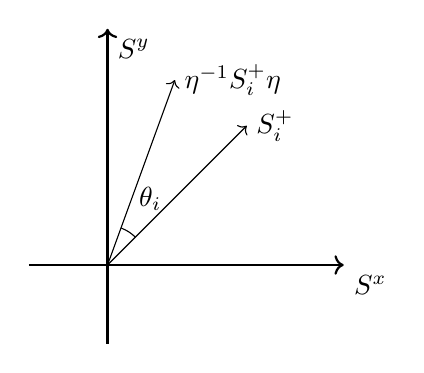
\begin{tikzpicture}
            \coordinate (origin) at (0,0);
            \coordinate (s) at (0.5,0.5);
            \coordinate (s_prime) at (0.3,0.8);
            \draw[thick,->] (-1,0) -- (3,0) node[anchor=north west] {$S^x$};
            \draw[thick,->] (0,-1) -- (0,3) node[anchor=north west] {$S^y$};
            \draw[->] (origin) -- (45:2.5) node [black,right] {$S_i^+$};
            \draw[->] (origin) -- (70:2.5) node [black,right] {$\eta^{-1}S_i^+\eta$};
            \pic[draw, "$\theta_i$", angle eccentricity=2] {angle = s--origin--s_prime};
        \end{tikzpicture}
    \end{column}
    \end{columns}
    \pause 
    \begin{align*}
        \eta^{-1} H \eta = H + J \sum_{i = -l}^{l-1} \left[e^{\frac{-i\pi}{l}} - 1 \right]  S^+_i S^-_{i+1} + \left[e^{\frac{i\pi}{l}} - 1 \right] S^-_i S^+_{i+1}
    \end{align*}

    \begin{align*}
        &\braket{\Psi_1|H - E_0|\Psi_1} = \braket{\Psi_0|\eta^{-1} H \eta -E_0|\Psi_0} \nonumber \\ 
        &= 2J \left[\cos(\frac{\pi}{l}) - 1 \right] \sum_{i=0}^{l-1} \braket{\Psi_0|S^+_i S^-_{i+1} + S^-_{i} S^+_{i-1}|\Psi_0} \nonumber \\ 
        &=  2 \pi^2 J e_0  \frac{1}{l} \ \alert{\textbf{Doesn't depend on spin.}}
    \end{align*}

\end{frame}

\begin{frame}
    \frametitle{$\braket{\Psi_1|\Psi_0} \rightarrow 0 $}
    We study the parity of the state $\ket{\Psi_1}$ as compared to the parity of the ground state $\ket{\Psi_0}$. Let the parity operator be $\mathcal{P}$. 
    \begin{align*}
        &\mathcal{P} H \mathcal{P}^{-1} = H \nonumber \\ 
        &\mathcal{P} \ket{\Psi_0} = \pm \ket{\Psi_0} \nonumber \\ 
        &\mathcal{P} \ket{\Psi_1} = \pm \mathcal{P} \eta \mathcal{P}^{-1} \ket{\Psi_0} 
    \end{align*}
    \pause 
    Using $\mathcal{P} S^z_i \mathcal{P}^{-1} = -S^z_{-i}$, 
    \begin{align*}
        \mathcal{P} \eta \mathcal{P}^{-1} = e^{i2\pi \sum_{i=-l}^{l} S^z_i} \eta \ = \left\{
        \begin{matrix}
            \eta && s \text{ integer} \\
            -\eta && s \text{ half integer} 
        \end{matrix}
        \right.
    \end{align*}
    
\end{frame}

\section{Solvable models and valence bond solid states}
\begin{frame}
    \frametitle{Majumdar-Gosh Model (a warm up)}
    For a spin-1/2 chain,
    \begin{align*}
        H = J \sum_ i (\vec{S}_{i} + \vec{S}_{i+1}  + \vec{S}_{i+2})^2 = J\sum_ i \vec{S}_{i} \cdot \vec{S}_{i+1}  +\frac{1}{2} \vec{S}_{i} \cdot \vec{S}_{i+2} 
    \end{align*}
    \pause 
    Adding 3 spin-1/2 gives either spin-3/2 or spin-1/2. 
    \pause 
    
    The ground state must have any adjacent 3 sites to have total spin of 1/2. 
    \pause 

    This can be achieved by paring adjacent spins into singlets. 
    \begin{figure}[h]
        \centering
        \subfigure[]
        {
        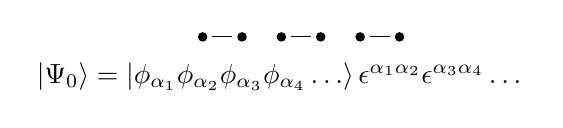
\begin{tikzpicture}
            \foreach \i in {0,...,5}
                {
                \draw[fill, black] (0.5*\i,0) circle (1.5pt) node[] (\i){};
                }
            \draw[black] (0) -- ( 1);
            \draw[black] (2) -- (3);
            \draw[black] (4) -- (5);
            \node [black] at (1,-0.5) {$\ket{\Psi_0} = \ket{\phi_{\alpha_1} \phi_{\alpha_2} \phi_{\alpha_3} \phi_{\alpha_4} \dots }\epsilon^{\alpha_1 \alpha_2} \epsilon^{\alpha_3 \alpha_4} \dots$};
        \end{tikzpicture}
        } \hfill
        \subfigure[]
        {
        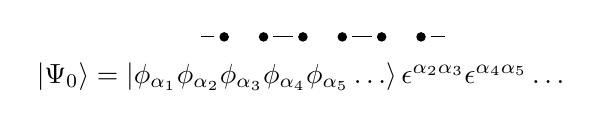
\begin{tikzpicture}
            \foreach \i in {0,...,5}
                {
                \draw[fill, black] (0.5*\i,0) circle (1.5pt) node[] (\i){};
                }
            \draw[black] (0) -- (-0.3,0) ;
            \draw[black] (1) -- (2);
            \draw[black] (3) -- (4);
            \draw[black] (5) -- (2.8,0) ;
            \node [black] at (1,-0.5) {$\ket{\Psi_0} = \ket{\phi_{\alpha_1} \phi_{\alpha_2} \phi_{\alpha_3} \phi_{\alpha_4} \phi_{\alpha_5} \dots }\epsilon^{\alpha_2 \alpha_3}\epsilon^{\alpha_4 \alpha_5}\dots$};            
        \end{tikzpicture}
        }
        \caption{Two ways adjacent spins can be paired into singlets.}
        \label{half_vbs}
    \end{figure}
\end{frame}

\begin{frame}
    \frametitle{Majumdar-Gosh Model}
    Remarks about the ground sates: 
    \begin{itemize}
        \item A contraction between 2 spin-1/2 into a spin singlet is called a valence bond. These ground states of the Majumadar-Gosh model are valence bond states with all the spins contracted. \pause 
        \item There are two ground states in consistency with LSM theorem. \pause 
        \item The ground states breaks translational symmetry. These states are fully dimerized. \pause
        \item These states has a very short correlation length, \begin{align*}
            \braket{\vec{S}_{i} \cdot \vec{S}_{j}} = 0 \ \  \text{for} \  |R_i-R_j| > 1
        \end{align*}\pause
        \item This suggest the existence of a gap.  
    \end{itemize}

\end{frame}

\begin{frame}
    \frametitle{Valence bond states} 
    The motivation for the next model came from trying to find a spin-1 Hamiltonian that has a valence bond state as its ground state. \pause 

    We need a way to generalize valence bond states to higher spins\pause 

    For spin-1 we think of each spin site as being made of 2 spin-1/2s. And always construct states that are symmetric in same site spin-1/2s. \pause 

    The following can be used as a basis on each site, 
    \begin{align*}
        &\ket{\phi_{\alpha_1\alpha_2}} = \ket{\phi_{\alpha_2\alpha_1}} = \frac{1}{\sqrt{2}}(\ket{\phi_{\alpha_1} \phi_{\alpha_2}} + \ket{\phi_{\alpha_2} \phi_{\alpha_1}}) \nonumber \\ 
        & \braket{\phi_{\alpha_1 \alpha_2} | \phi_{\beta_1 \beta_2}} = \delta_{\alpha_1 \beta_1} \delta_{\alpha_2\beta_2} + \delta_{\alpha_1\beta_2}\delta_{\alpha_2\beta_1}
    \end{align*}
\end{frame}

\begin{frame}
    \frametitle{Valence bond states}
    Let's look at the possible valence bond states of spin-1 chain. 
    \begin{figure}[h]
        \centering
        \subfigure[]
        {
        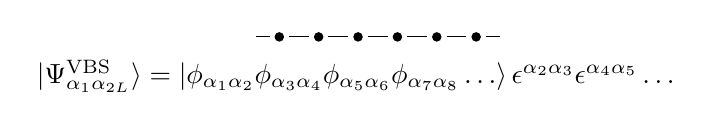
\begin{tikzpicture}
            \foreach \i in {0,...,5}
                {
                \draw[fill, black] (0.5*\i,0) circle (1.5pt) node[] (\i){};
                }
            \draw[black] (0) -- (-0.3,0) ;
            \draw[black] (0) -- (1);
            \draw[black] (1) -- (2);
            \draw[black] (2) -- (3);
            \draw[black] (3) -- (4);
            \draw[black] (4) -- (5);
            \draw[black] (5) -- (2.8,0) ;
            \node [black] at (1,-0.5) {$\ket{\Psi^{\text{VBS}}_{\alpha_1 \alpha_{2L}}} = \ket{\phi_{\alpha_1 \alpha_2} \phi_{\alpha_3 \alpha_4} \phi_{\alpha_5 \alpha_6} \phi_{\alpha_7 \alpha_8} \dots }\epsilon^{\alpha_2 \alpha_3} \epsilon^{\alpha_4 \alpha_5} \dots$};
        \end{tikzpicture}
        } \hfill
        \subfigure[]
        {
        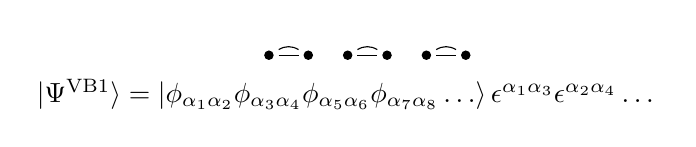
\begin{tikzpicture}
            \foreach \i in {0,...,5}
                {
                \draw[fill, black] (0.5*\i,0) circle (1.5pt) node[] (\i){};
                }
            \draw[black] (0) -- (1);
            \draw[bend left]  (0) to node [auto] {} (1);
            \draw[black] (2) -- (3);
            \draw[bend left]  (2) to node [auto] {} (3);
            \draw[black] (4) -- (5);
            \draw[bend left]  (4) to node [auto] {} (5);
            \node [black] at (1,-0.5) {$\ket{\Psi^{\text{VB1}}} = \ket{\phi_{\alpha_1 \alpha_2} \phi_{\alpha_3 \alpha_4} \phi_{\alpha_5 \alpha_6} \phi_{\alpha_7 \alpha_8} \dots }\epsilon^{\alpha_1 \alpha_3}\epsilon^{\alpha_2 \alpha_4}\dots$};            
        \end{tikzpicture}
        }
        \subfigure[]
        {
        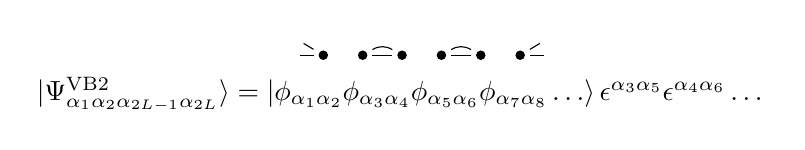
\begin{tikzpicture}
            \foreach \i in {0,...,5}
                {
                \draw[fill, black] (0.5*\i,0) circle (1.5pt) node[] (\i){};
                }
            \draw[black] (0) -- (-0.3,0) ;
            \draw[black] (0) -- (-0.25,0.15);
            \draw[black] (1) -- (2);
            \draw[bend left]  (1) to node [auto] {} (2);
            \draw[black] (3) -- (4);
            \draw[bend left]  (3) to node [auto] {} (4);
            \draw[black] (5) -- (2.8,0);
            \draw[black] (5) -- (2.75,0.15);
            \node [black] at (1,-0.5) {$\ket{\Psi^{\text{VB2}}_{\alpha_1\alpha_2\alpha_{2L-1}\alpha_{2L}}} = \ket{\phi_{\alpha_1\alpha_2} \phi_{\alpha_3 \alpha_4} \phi_{\alpha_5 \alpha_6} \phi_{\alpha_7 \alpha_8} \dots }\epsilon^{\alpha_3 \alpha_5}\epsilon^{\alpha_4 \alpha_6}\dots$};            
        \end{tikzpicture}
        }
        \caption{3 possible valence bond states. (a) is the VBS partially dimerized state. (b) and (c) are the fully dimerized states.}
        \label{one_vbs}
    \end{figure}

\end{frame}

\begin{frame}
    \frametitle{AKLT model}
    The AKLT model is a spin-1 chian model with the VBS state being the ground state, 
    \begin{align*}
        H &= 2J\sum_i P^{(2)}(\vec{S}_{i} + \vec{S}_{i+1} ) \nonumber \\
          &= J\sum_i \frac{1}{12} (\vec{S}_{i} + \vec{S}_{i+1} )^2 ((\vec{S}_{i} + \vec{S}_{i+1} )^2 -2) \nonumber \\ 
          &= J \sum_i \vec{S}_{i} \cdot \vec{S}_{i+1} + \frac{1}{3} (\vec{S}_{i} \cdot \vec{S}_{i+1})^2 + \text{const.}
    \end{align*}
    \pause 
    This Hamiltonian is positive definite, the ground state will have $E_0 = 0$. \pause
    
    The VBS state has for every 2 adjacent spin sites 2 of the 4 spin-1/2s to be contracted into a spin singlet. \pause 
    
    Hence the total spin of any 2 adjacent spin sites cannot be 2 with only 2 spin-1/2s left. This shows the VBS state to be a ground state.
    

\end{frame}

\begin{frame}
    \frametitle{AKLT model}
    \begin{align*}
        H \ket{\Psi_{\text{VBS}}} = 0 
    \end{align*}
    \pause 
    What is more subtle is to show that this is the only ground state! \pause 
    It is the unique ground state up to some boundary modification. \pause
    \begin{center}
        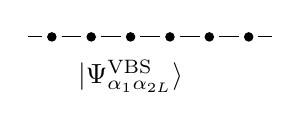
\begin{tikzpicture}
            \foreach \i in {0,...,5}
                {
                \draw[fill, black] (0.5*\i,0) circle (1.5pt) node[] (\i){};
                }
            \draw[black] (0) -- (-0.3,0) ;
            \draw[black] (0) -- (1);
            \draw[black] (1) -- (2);
            \draw[black] (2) -- (3);
            \draw[black] (3) -- (4);
            \draw[black] (4) -- (5);
            \draw[black] (5) -- (2.8,0) ;
            \node [black] at (1,-0.5) {$\ket{\Psi^{\text{VBS}}_{\alpha_1 \alpha_{2L}}} $};
        \end{tikzpicture}
    \end{center}
    \pause 
    One can get around this by considering an infinite system, or to be more concrete, study the system under periodic boundary conditions. 
    \begin{center}
        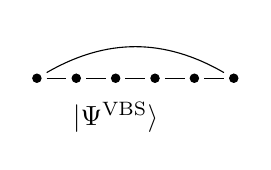
\begin{tikzpicture}
            \foreach \i in {0,...,5}
                {
                \draw[fill, black] (0.5*\i,0) circle (1.5pt) node[] (\i){};
                }
            \draw[black] (0) -- (1);
            \draw[black] (1) -- (2);
            \draw[black] (2) -- (3);
            \draw[black] (3) -- (4);
            \draw[black] (4) -- (5);
            \draw[bend left]  (0) to node [auto] {} (5);
            \node [black] at (1,-0.5) {$\ket{\Psi^{\text{VBS}}} $};
        \end{tikzpicture}
    \end{center}


\end{frame}


\begin{frame}
    \frametitle{Correlation length of the VBS state}
    \begin{align*}
        \vec{S}\ket{\phi_{\alpha_1\alpha_2}} = \frac{1}{2}(\vec{\sigma}_{\beta \alpha_1} \ket{\phi_{\beta \alpha_2}} + \vec{\sigma}_{\beta \alpha_2} \ket{\phi_{\alpha_1\beta}} ) 
    \end{align*}
    \begin{align*}
        \braket{\vec{S}_i \cdot \vec{S}_j} = 4 (-1)^{R_j - R_i} 3^{-|R_j - R_i|}
    \end{align*}

    \begin{align*}
        \xi = \frac{1}{\log 3} = 0.9
    \end{align*}
    \pause 
    Finite length correlation function suggests the existence of a gap. 
    \pause 

    Numerical results shows that the VBS state has energy that is only 5\% higher than the ground state of the Heisenberg Hamiltonian. 
    \pause 

    Correlation length does agree as much. Numerical results suggests $\xi = 5$. 
\end{frame}

\begin{frame}
    \frametitle{Trivia}
    Looking on the more general Hamiltonian, 
    \begin{align*}
        H = J \sum_i \vec{S}_{i} \cdot \vec{S}_{i+1} - \beta (\vec{S}_{i} \cdot \vec{S}_{i+1})^2
    \end{align*}
    there is another solvable point at $\beta = 1$, which is gapless. 
    \pause 

    The model with $\beta = 1$ was solved by Bethe in the 1930s. 
    \pause 
    \begin{columns}
    \begin{column}{0.3\textwidth}
        A phase transition occur at $\beta = 1$. 
        \pause 

        The graphs suggests that the phase transition occur between the VBS and the dimerized state.
    \end{column}
    \begin{column}{0.7\textwidth}
        \begin{figure}[h]
            \centering
            \includegraphics[scale=0.4]{tmp_z_h7tj6o.png}
        \end{figure}
    \end{column}
    \end{columns}
    


    

\end{frame}

\section{Symmetry of the VBS state}
\begin{frame}
    \frametitle{Symmetry of VBS state}
    No local order parameter characterizes the transition to the VBS state. \pause

    The periodic VBS chain preserve all local symmetries of the Hamiltonian like rotation, inversion, translation, and time reversal symmetry. 
    \pause 
    
    This here is an example of a symmetry protected topology. 
    Let's study the VBS state with open boundary condition.     
    \begin{center}
        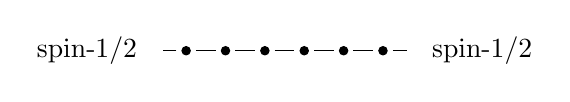
\begin{tikzpicture}
            \foreach \i in {0,...,5}
                {
                \draw[fill, black] (0.5*\i,0) circle (1.5pt) node[] (\i){};
                }
            \node [black,left] at (-0.5,0) {spin-1/2};
            \draw[black] (0) -- (-0.3,0) ;
            \draw[black] (0) -- (1);
            \draw[black] (1) -- (2);
            \draw[black] (2) -- (3);
            \draw[black] (3) -- (4);
            \draw[black] (4) -- (5);
            \draw[black] (5) -- (2.8,0) ;
            \node [black,right] at (3,0) {spin-1/2};
            
        \end{tikzpicture}
    \end{center}
The state has 2 "free" spin-1/2, one at each end of the chain, that transforms differently as compared to the bulk. \pause 

Such a weird situation at the boundaries can only be changed by a transformations that mixes the boundaries. \pause 

Such along range correlation between the ends of the chain can only happen if the bulk closes a gap. 
\end{frame}

\end{document}